\newcommand{\minus}{\scalebox{0.65}[1.0]{$-$}}
\renewcommand*\descriptionlabel[1]{\hspace\leftmargin$#1$}
\setcounter{tocdepth}{5}
\setcounter{secnumdepth}{5}

%\section{Energy}

%In modern society, the usefulness and convenience supplied by advancing technologies has allowed quality of life to increase drastically over time. Within these advancing technologies, ranging from air conditioning to food production, there is a common thread of energy requirement. To cool the air, energy is required in order to compress, pressurize, and cool the refrigerant. To produce food, energy is required to pump water, create fertilizer, and operate heavy machinery. Thus, the importance of energy is significant in maintaining and developing quality of life for society.

%However, energy is not free, and it takes effort to harvest and convert energy into usable forms. For wind power, this means building large turbines which can be turned by the wind. For solar power, this means building solar panels, which convert photons from the sun into electrical energy. However, for most large-scale electrical generation needs, it is more efficient for the conversion aspect to use boiling water to turn a turbine, which then generates electricity, as can be seen in Figure \ref{fig:energy-gen-methods}. Regardless of how it is generated, electricity can then be transported or stored to be used by people for any variety of purpose.

%\begin{figure}[H]
%  \centering
%  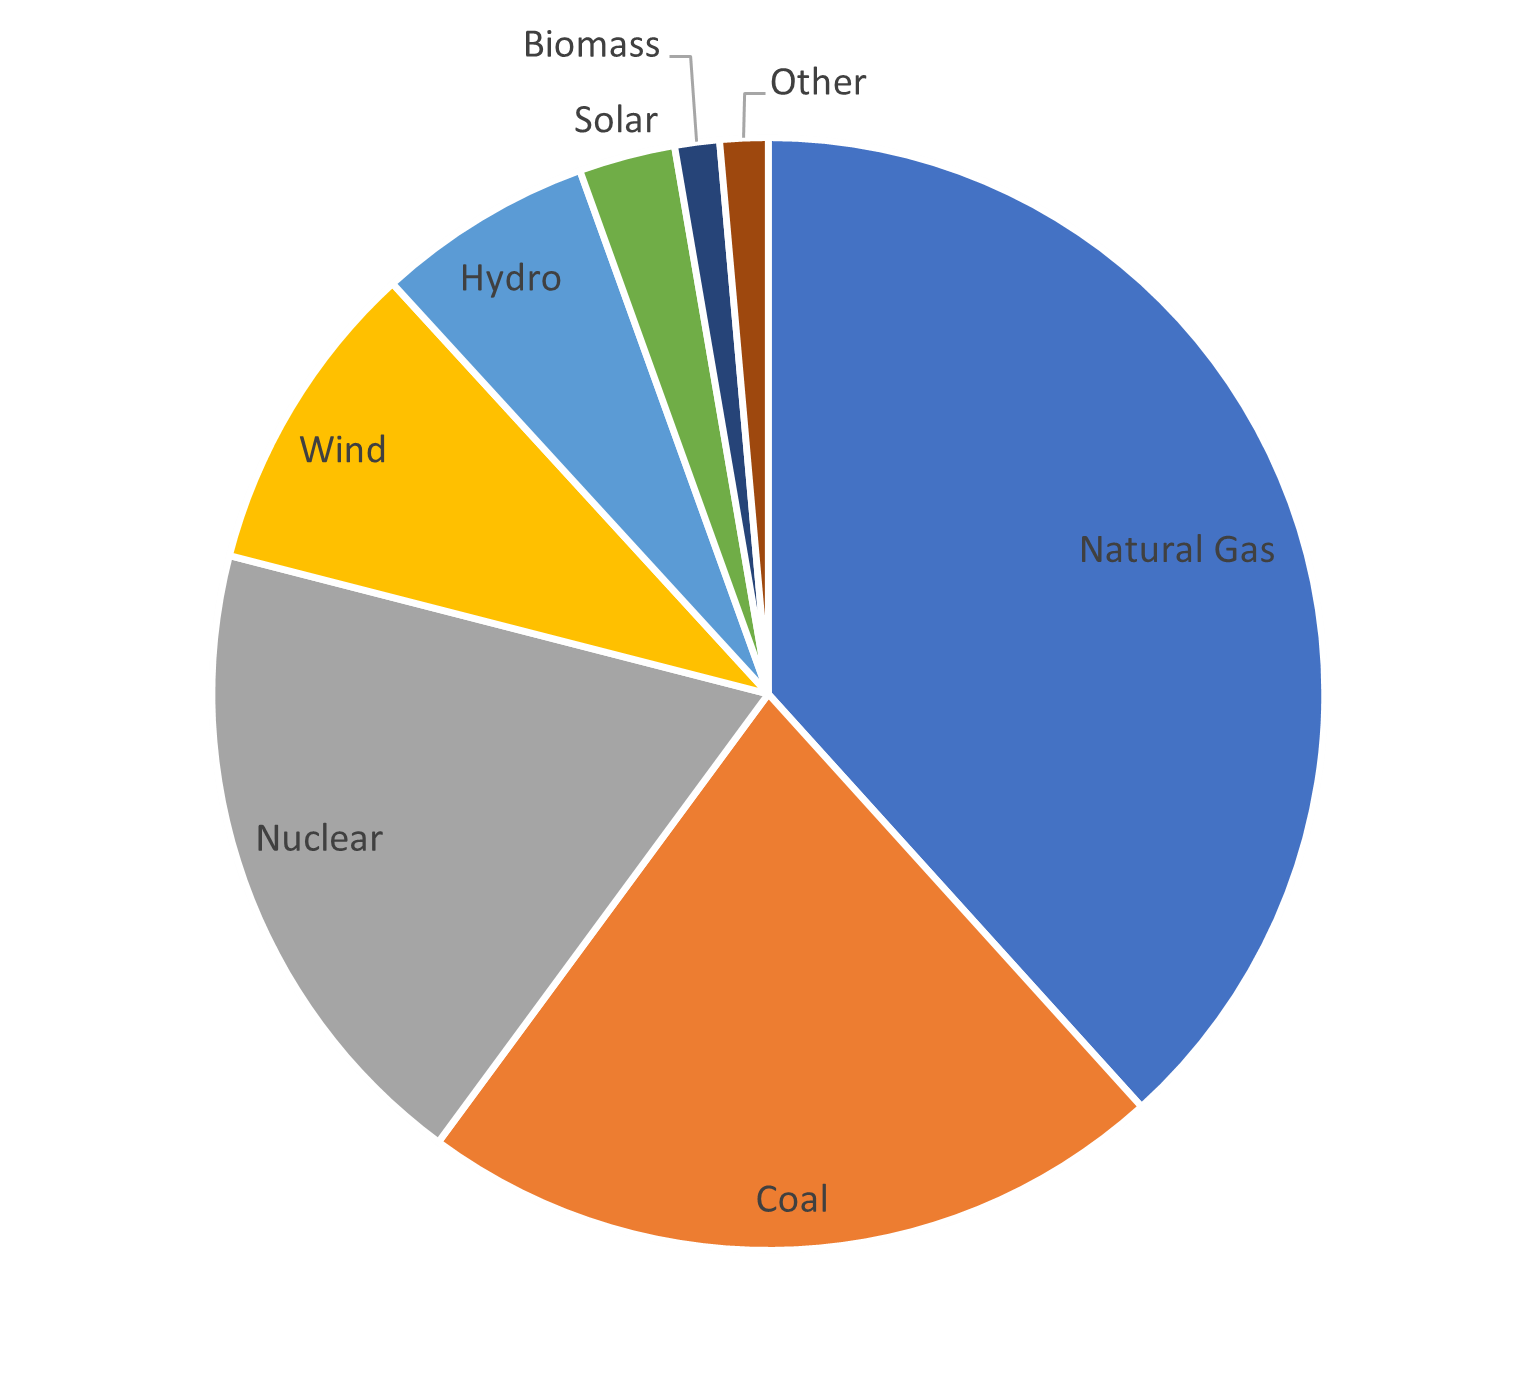
\includegraphics[scale=0.7]{images/US-energy-prod.png}
%  \caption{Energy generation in the United States in 2021 from the US %Energy Information Administration CITE %https://www.eia.gov/electricity/monthly/.}
%   \label{fig:energy-gen-methods}
%\end{figure}

%Figure \ref{fig:energy-gen-methods} shows the portion of energy generation. From this figure, it can be seen that the methods which dominate energy contribution are natural gas, coal, and nuclear. Of the various methods to generate electricity, desirable characteristics would be safety, efficiency, consistency, availability, and economics. Nuclear energy is strong in these characteristics, though there is an economic problem due to high up-front costs, which are on the order of \$10 billion for a 1GW nuclear power plant \cite{du_update_2009}.

%\section{Nuclear Energy}

%Part of the reason nuclear energy has high up-front costs is because the nuclear industry is highly safety conscious and has many regulations in place in order to minimize risks. Although this mindset increases costs, the effort has paid dividends, which is apparent when viewing the deaths associated with different energy generation methods, shown in Table \ref{tab:death-mega} \cite{brook_why_2014}.

%\begin{table}[H]
%\renewcommand{\arraystretch}{1.25}
%\caption{Mortality rates for each energy source in deaths per billion kWh %produced (recreated from \cite{brook_why_2014}).}
%\label{tab:death-mega}
%\begin{center}
%\begin{tabular}{ | c | c | }
% \hline
% Energy Source & Mortality Rate (deaths per billion kWh)\\
% \hline
% \hline
% Coal (Global Average) & 100 \\
% Biofuel/Biomass & 24 \\
% Coal (U.S.) & 15 \\
% Oil & 36 \\
% Natural Gas & 4 \\
% Hydro (Global Average) & 1.4 \\
% Solar (Rooftop) & 0.44 \\
% Wind & 0.15 \\
% Nuclear (Global Average) & 0.04 \\

% \hline
%\end{tabular}
%\end{center}
%\end{table}

%Even though the up-front costs are high, nuclear power plants are licensed to operate for 40 years and can get extensions to extend that time by 10-20 years \cite{bredimas_international_2008}. This means that nuclear plants are a very long term investment. An investment at this time scale is difficult to make for a private industry though, as there is less risk when investing in cheaper plants, such as natural gas.

%In order to address the economic issue of nuclear power plants, there are many different approaches which are implemented. One of these is to build smaller, cheaper nuclear plants which are then more affordable and are have less up-front cost. Another approach is from the regulation perspective, and involves either taxing negative externalities more harshly or subsidizing carbon-free energy sources. There is also the approach of developing new generation IV reactor designs \cite{kelly_generation_2014}.

% Why MSRs, why depletion

\section{Molten Salt Reactors}

One of the generation IV reactor designs is the molten salt reactor, or MSR \cite{kelly_generation_2014}.
In this work, the main MSR which will be discussed is the liquid fueled MSR. Moving forward, the term MSR will refer to the liquid fueled variant unless specified otherwise.
The MSR is an advanced reactor design which is intended to improve safety and efficiency over previous reactor designs.
%For example, the operating pressure in an MSR kept close to atmospheric while the temperature is higher than that of traditional light water reactors.
%The lower pressure is useful from a safety perspective, while high temperatures with the high thermal capacity and conductivity of molten salts allows for high efficiency.



%The MSR potentially offers a lower "n'th-of-a-kind" cost of electricity when compared to coal and pressurized water reactors, which are a large portion of the nuclear fleet \cite{moir_cost_2002}.
%Of particular interest in this thesis is the liquid fueled MSR design, which is significantly different from the current light water reactor, or LWR, designs which dominate the nuclear fleet currently in use.
%Light water reactors include boiling water reactors (BWRs) and pressurized water reactors (PWRs), both of which are well understood reactor designs currently implemented.
%Light water reactors use a solid fuel containing uranium-235 with a water coolant, which also serves as a moderator to slow down the neutrons to thermal energies. This fuel generates heat as the fissile uranium-235 fissions. After some lengthy amount of depletion, it can be reshuffled or removed from the reactor to be placed into a cooling pool.

MSRs, instead of a solid fuel, use a liquid fuel composed of a molten salt mixed with some fissile isotope, such as uranium-235. Some of the benefits of MSRs include high operating temperature, low operating pressure, and high thermal conductivity and capacity of the salts. Other benefits include a high coefficient of thermal expansion for negative temperature coefficient of reactivity, high resource utilization through higher burn-up, reduced cost of fabricating and transporting fuel elements, and the removal of fission products to improve the neutron economy \cite{serp_molten_2014}.
% WHy MSRs? How will it help nuclear? Reactivity/power density?

MSRs also have several barriers to deployment which must be handled. Corrosion and material degradation is an issue for MSRs, as the high temperature salts are highly corrosive. Another barrier to deployment is in regulation, as the MSR operates very differently from traditional reactors. In order to properly regulate MSRs, it is important to have models which are able to simulate them correctly. One type of simulation which is important for determining fuel composition and reactor properties after long periods of operation are depletion simulations, which are of key interest for this work.

\section{Physical Depletion and Reprocessing}

%In a depletion simulation, general data is generated about the model at each depletion time step. After each of these steps, updated data is then used for the next depletion step. This updated data includes cross section data, energy spectra, neutron flux, and can include changes to temperature, volume, densities, or compositions. For MSRs, these updated changes after each depletion step need to account for the effects of online reprocessing.

Depletion is the process of fission over time, leading to fission products and decay chains. For an MSR with online reprocessing, the additions and losses from reprocessing have to be considered within depletion.

Continuous reprocessing is a process which involves adding fresh fuel to the system, as well as chemically removing fission products. MSRs are also capable of batchwise reprocessing, which is a process which occurs in discrete steps, such as salt disposal after some set amount of time. Typically, most reprocessing schemes suggest continuous reprocessing while the reactor is online.

The usefulness of reprocessing, particularly online reprocessing, is that the reactor does not need excess reactivity in order to continue operating for a long period of time. In a typical light water reactor, burnable poisons and control rods are used to lower reactivity at the beginning of the core life so the reactor can remain at a safe critical level over the core life. In an MSR, the parasitic absorbers, such as xenon-135, can be removed from the reactor to further improve the neutron economy. Additionally, fresh fuel salt can be added to the reactor in order to maintain stable operation.

The fresh fuel feed can include fissile isotopes, such as uranium-233 or uranium-235, fertile isotopes, such as uranium-238 or thorium-232, or some combination of both. Adding a fissile isotope to the reactor will allow the reactor to continue operating as is. For the fertile isotopes, the neutron first absorbs a neutron, then the product of that reaction decays and produces a fissile isotope. This process is illustrated for thorium-232 breeding in Equation \eqref{eq:th-pa-chain}, which is the breeding process used in the Molten Salt Breeder Reactor (MSBR). By using a balance of fissile and fertile feeds, the reactor can breed new fuel while it continues to safely operate.

\begin{equation} \hfill
\ce{^{232}_{90}Th} + \ce{^{1}_{0}n} \longrightarrow \ce{^{233}_{90}Th} \longrightarrow \ce{^{233}_{91}Pa} \longrightarrow \ce{^{233}_{92}U}
\hfill\label{eq:th-pa-chain} \end{equation}

The half life of thorium-233 via beta decay is on the order of tens of minutes, while the half life of protactinium-233 via beta decay is roughly 27 days.
%Without reprocessing, the protactinium-233 remaining in the core for such a period of time would be more likely to interact with neutrons, impacting the breeding efficiency.
If the protactinium-233 remains in the core, it will be removed by competing processes of decay and neutron absorption.
This will impact the breeding efficiency.
To minimize this, the MSBR continuously chemically extracts the protactinium from the fuel salt, allowing it to decay in a separate tank until it decays into a fissile fuel.
Once it has decayed, another continuous chemical process removes the fissile fuel from the tank and reloads it into the reactor.
%another continuous chemical process strips uranium which is formed and brings the uranium back into the reactor, continuing the process.

Overall, in MSR reprocessing, the two different physical approaches are continuous and batchwise. The reprocessing schemes can be online, while the reactor is operating, or offline, when the reactor is shutdown. Of particular importance for MSR behaviour is online reprocessing, which changes the fuel composition while the reactor is operating. This means that an important type of model for MSR analysis is a depletion simulation which handles the effects of online reprocessing.

\section{Computational Depletion and Reprocessing}

The depletion simulation itself can be performed using a stochastic method, such as Monte Carlo, or a deterministic method, such as diffusion. This depletion simulation alone will only provide inform on the MSR without consideration for the reprocessing.

%An important type of model to simulate for reactor analysis is a depletion model, where the reactor operates for some length of time using discrete depletion steps. This model is important to determine fuel utilization, neutronic parameters at different stages in the reactor life, and to make further decisions about the reactor.

%In a depletion simulation, general data is generated about the model at each depletion time step. After each of these steps, updated data is then used for the next depletion step. This updated data includes cross section data, energy spectra, neutron flux, and can include changes to temperature, volume, densities, or compositions. For MSRs, these updated changes after each depletion step need to account for the effects of online reprocessing.

In order to model online reprocessing in a depletion simulation, there are two different computational methods which can be implemented. These methods reflect the physical continuous and batchwise reprocessing methods and have the same naming convention. However, it is fairly common for MSR simulations with a continuous reprocessing scheme to use approximate batchwise mathematical models.

In this work, I will compare and investigate the differences between continuous and batchwise computational reprocessing methods.
Because the effects of depletion and reprocessing are temporal, I will vary the depletion step size.
I will compare the validity of batchwise methods approximating continuous methods, and I will quantify the effects of different sub-methods within both batchwise and continuous.
%This investigation involves effects of depletion step size, validity of batchwise methods approximating continuous methods, and different sub-methods within both batchwise and continuous methods which can be implemented.

